\chapter{Introduction Générale}
\pagebreak

Depuis les années 1950, on parle d'intelligence artificiel (IA, ou AI en anglais) un processus ayant les capacités de penser ou de raisonner comme une tache qui serait humainement exécuté a l'aide d'une conscience ou un réseau neuronal. Un processus pensant pouvant prédire une action, un état ou un résultat. Mais l'intelligence artificiel est en réalité plus complexe que sa, un processus pouvant donner des résultats sur des données qu'elle connait et donc que le processus connait à l'avance le résultat n'est pas un processus d'intelligence artificiel car elle ne fait que pour un dictionnaire de données retourner la valeur associé aux data donné. \\
Pour qu'un processus soit dit, doté d'une intelligence, il faut qu'elle soit équipé d'une capacité de raisonnement voir d'apprentissage pour les cas où les données donné en entré soit totalement inconnue du processus, dans ce cas la le processus doit savoir prédire une réponse viable et ayant du sens en utilisant les données qu'elles connait déjà.\\
\linebreak
Le domaine de l'intelligence artificiel est bien plus vaste que la description donné ci dessus, selon le \textit{Texte de la 236e conférence de l'université de tout les savoirs donné par Jean-paul HALTON} il existerai 3 grandes approches à l'intelligence artificiel, l'approche \emph{Symbolique}, l'approche \emph{Connexioniste} puis l'approche \emph{Statistique}, ces trois termes sont décrit ci dessous.

\pagebreak
\section{L'approche symbolique}

Un exemple réelle d'approche symbolique serait dans le code de la route, chaque panneaux (ou inscriptions qu'elles soient au sol ou peu importe où) ont une signification spécifique sur l'état que l'automobiliste doit adopter sur certain tronçon de route ou dans un état future. Si un automobiliste voit un panneau <sens interdit> sur un tronçon juste devant lui, une information est envoyé au cerveaux (où plutôt dans la base de connaissance) et une réponse direct (sans aucun apprentissage) est retourné par le réseau de connaissance indiquant qu'il ne faudrait pas aller sur ce tronçon sous resserve d'accidents par exemple.\\
Cette approche est dit \textbf{offline} car avant d'effectuer des requêtes à la base de connaissance celle ci a besoin d'être au préalable remplit d'informations vrai et de tout les cas possible. Admettons qu'un conducteur n'ai pas apprit la signification d'un panneau <sens interdit> voyer vous le problème que cette individu peut causer.\\
L'hypothèse du monde clos est appliqué par cette approche, pour une donné que le réseau de connaissance ne connais pas, la réponse retourné sera une réponse négative, prenons encore notre conducteur ci dessus, si celui ci voit un nouveau tronçon devant lui (un tronçon qu'il n'a jamais vue), il n'a aucune données dans sa base de connaissance qui décrit ce nouveau tronçon (bien-sur nous allons admettre que le conducteur n'a pas la possibilité d'ajouter de nouvelles informations dans sa base de connaissance ni d'apprendre sur ce nouveau tronçon), le conducteur va trivialement dire qu'il ne va pas s'aventurer sur ce nouveau tronçon car sa base de connaissance n'a pu fournir aucune informations sur ce telle tronçon. \\
\linebreak
Dans l'informatique, nous le savons, les ordinateurs ne savent que faire des opérations logique simple comme le ET, le OU, et le NOT, ces opérations sont accompagné de registres (mémoire vive, disque dur, ...) pouvant pour la duré de la vie d'un processus stocker les données et faire des opérations dessus avec d'autres données stocké dans la machine, c'est de la qu'avec quelques registres et une succession d'opérations logiques simple on peut former des circuits pouvant traiter les opérations mathématiques comme l'addition, la soustraction, la multiplication et la division.
Ses informations sont possibles car elles sont ancré dans la base de connaissance de la machine qui lance les processus, par héritage les processus sont capable d'appeler les circuits pouvant faire les opérations cité ci dessus. \\
Un exemple logiciel d'approche symbolique serait le langage \textit{Prolog} qui pour une base de connaissance donné en début de fichier, infère les différents questions posé dans la suite du programme.\\
Prenons un exemple simple, pour une base de connaissance donné ci dessous:
\linebreak
\lstset{style=mlpythoncode}
\begin{lstlisting}[language=Prolog]
- Homme(Jean)
- Homme(Pierre)
- Femme(Marie)
- En_couple(Jean,Marie)
\end{lstlisting}
\ \\
Effectuons des requêtes à la base de donnée ci dessus, demandons:
\begin{description}
\item[] Es ce que Jean est un homme? la base de connaissance va répondre oui.
\item[] Es ce que Marie est un homme? non.
\item[] Es ce que Marie et Pierre sont en couple? non.
\item[] Es ce que Jean et Marie sont en couple? oui.
\end{description}

Pour confirmer la théorie du monde clos, nous pouvons demander si Philippe et un homme, n'ayant aucune informations sur un dénommé Philippe, la base de connaissance va déclencher une exception disant qu'il n'a pas trouvé un tel Philippe, vu qu'il ne connais pas ce Philippe, la base de connaissance va répondre NON.\\
\linebreak
L'hypothèse du monde clos est une échappatoire fréquemment utilisé dans les bases de connaissances, mais le non envoyé à cause de cette hypothèse n'a pas la même signification que le non Philippe n'est pas une homme. Pour y remédier certain logiciels ont ajouté une valeur à "oui" et "non", nous appelons ceci le \textit{Three valued logic} et ce mode est implémenté dans certaines bases SQL, la troisième valeur est nommé "unknow" ayant la bonne signification demandé par l'hypothèse du monde close.

\pagebreak
\section{L'approche connexionniste}
L'approche connexionniste est l'approche la plus proche du schéma du cerveaux au vue de requêtes. Le processus de réflexion du cerveau est représenté par une série de mini processus ne pouvant répondre qu'a un type de problème qui est définit lors de la création de ce mini processus, un mini processus est nommé neurone dans le cerveau, et nous allons préférer l'utilisation du terme neurone pour la suite. \\
Chaque neurone est définit par plusieurs entrées, et une seul sortie et peu être semblable à un \textit{Perceptron} en machine learning:

\begin{center}
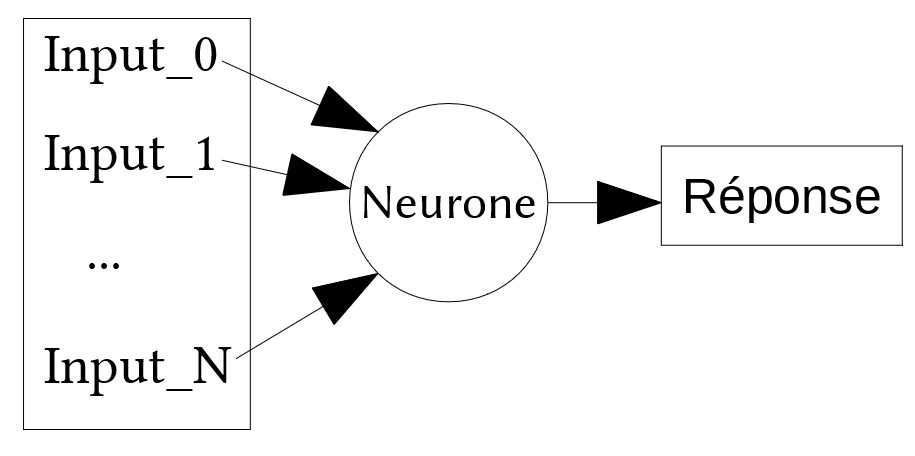
\includegraphics[scale=0.3]{img/neurone.jpg} 
\end{center}

